\documentclass[10pt, twocolumn, twoside]{article}

\usepackage{graphicx}
\usepackage{amsmath, amssymb}
\usepackage{enumerate}
\usepackage{titleps}
\usepackage[top=1.25in,bottom=1in,right=1in,left=1in]{geometry}
\usepackage[parfill]{parskip}
\usepackage{titling}
\usepackage{hyperref}
\usepackage[authoryear]{natbib}

\newpagestyle{ruled}
{\setfoot{}{\thepage}{} \footrule}
\pagestyle{ruled}


\setlength{\droptitle}{-4em}   % This is your set screw
\posttitle{\par\end{center}\vskip 0.5em}


\title{Bayesian Reinforcement Learning}
\date{}
\author {Vickie Ye and Alexandr Wang}


\begin{document}
\maketitle

\section{Introduction}
In reinforcement learning, the learning procedure consists of two parallel processes:
estimating parameters of the surrounding environment and learning the optimal policy
of highest long-term reward. A common way this is done is by learning a latent ``value''
function over the states and actions, which the agent uses to make policy decisions.

In this project, we examined two Bayesian approaches to learning the latent value function
and policy. One way to do this is with a Bayesian model to estimate the parameters of the
environment, as done in \cite{strens}. This framework places Bayesian priors on the
transition function and reward function of the environment and updates its posterior
as it interacts with the environment. 

Another Bayesian approach toward learning the value function uses Gaussian processes, as
in \cite{engel}. This approach to value function approximation is non-parametric, and
provides both a function estimate (the GP mean) and uncertainty (the GP covariance).
The flexibility of this framework allows it to scale well to harder, higher-dimensional
problems.

\section{Bayesian MDP}
MDPs are commonly used to learn the policy for the system with a set of states $S$,
a set of actions $A$, a reward function $R(S, A)$, and a transition function
$T(s, a, s') = P(X^{(t+1)} = s' | X^{(t)} = s, Y^{(t)} = a)$. To learn the optimal
long-term-reward policy, we define a quality function with discount factor
$\gamma$, $Q = \sum_{t=0}^\infty \gamma^t R^{(t)}$, which we approximate for each
state-action pair as
\begin{equation*}
Q(s, a) = \mathbb{E}[R(s,a)]+\gamma\sum_{s'}T(s, a, s')\textrm{max}_{a'} Q(s',a')
\end{equation*}

In this framework, the quantities we need to estimate are the reward function
$R(s, a)$ and transition probabilities $T(s, a, s')$ to make our updates to $Q$.

\subsection{Models for Transition Probabilities and Expected Return}
We define the transition distribution $\pi$ for each state-action pair $(s, a)$ as
\begin{equation*}
\mathbf{\pi}(s, a) = (T(s, a, s_0), ..., T(s, a, s_{N-1})),
\end{equation*}
where $\pi(s, a)_i = \mathbb{P}(s_i| s, a)$.

For our experiments we use a uniform Dirichlet prior with $\alpha_i = 1$.
Our updated posterior $\mathbf{\pi}(s, a)$ given the data is then
\begin{equation*}
\mathbf{\pi}^{(t)} \sim \textrm{Dirichlet}(\mathbf{\alpha}^{(t)}| \mathbf{m}^{(t)}),
\alpha^{(t)}_i = \alpha_i + m_i^{(t)}
\end{equation*}
where $\mathbf{m}^{(t)}$ represent the observed counts for the transitions. Then in estimating $Q$ at each time step, we sampled $\pi(s, a)$ from our posterior.

We represent the reward for each state-action pair $(s, a)$ as Gaussian-
distributed with mean $\mu$ and precision $\tau$. We use a Ga($\beta,\rho$)
prior for $\tau$ and a $\mathcal{N}(\mu_0, c_0\tau)$ prior for $\mu$. Then our
updated posteriors are
$$\tau \sim \textrm{Ga}\Big(\beta + \frac{k}{2}, \rho + \frac{1}{2}\sum_i(r_i - \bar{r})^2
+ \frac{kc_0(\bar{r}-\mu_0)^2}{2(n+c_0)}\Big),$$
$$\mu \sim \mathcal{N}\Big(\frac{k\bar{r} + c_0\mu_0}{k + c_0}, (k+c_0)\tau\Big)$$
for observed rewards $\mathbf{r} = \{r_i\}_{1\le i \le k}$ for the state-action pair.
Then in estimating $Q$ at each time step, we sampled $\mu$ and $\tau$, which we then used
to sample $R$, for each $(s, a)$.
For comparison we also evaluated performance when using the modes of the posterior as
estimates for $\pi(s, a)$ and $R(s,a)$.

\subsection{Testing Problems}
We used three toy problems to test our implementation. In the ``Chain'' problem
(Figure ~\ref{fig:chainloop} top), there are five states and two possible actions, with 0.2
probability of slipping (performing the opposite action intended). The optimal
policy is to explore to state 5, and stay there until slipping; the agent should try
to get back to state 5 as much as possible.

In the ``Loop" problem (Figure ~\ref{fig:chainloop} bottom), there are nine states and
two possible actions, with no possibility of slipping. The optimal policy is to stay
in the left loop and receive reward of 2 for every 5 actions. Because this problem has
very little distinguishing the two actions in terms of short-term reward, effective
estimation of $Q$ parameters is important to optimal behavior.

In the ``Maze'' problem (Figure ~\ref{fig:maze}), the agent explores a maze to find
flags. The agent can either move north, west, south, or east, and receives only its
current position as its state (it has no physical sensors or observations of walls,
besides the its new state). Each time the agent reaches the goal, it receives a reward
equal to the number of flags collected and is transported back to the beginning of the
maze. All other state-action pairs receive zero reward. In the maze problem, we also
have a probability of slipping (performing an action other than the one specified) of 0.2.

\begin{figure}[!htb]
\centering
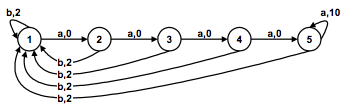
\includegraphics[width=0.4\textwidth]{chain.png}
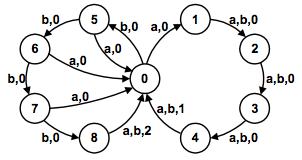
\includegraphics[width=0.4\textwidth]{loop.png}
\caption{\label{fig:chainloop} The ``Chain'' and ``Loop'' toy problems used in testing.}
\end{figure}

\begin{figure}[!htb]
\centering
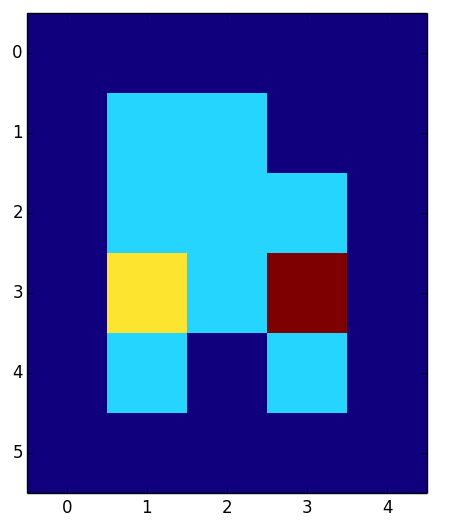
\includegraphics[width=0.18\textwidth]{easymaze.png}
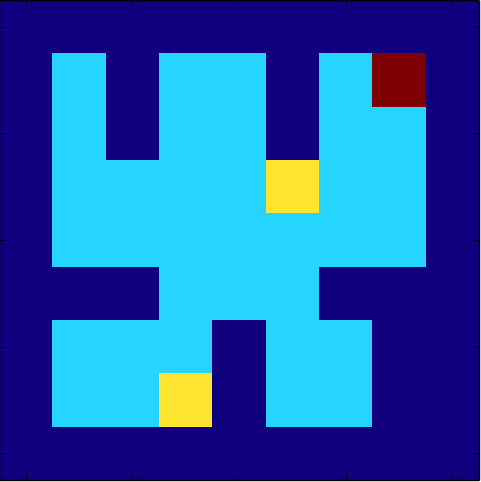
\includegraphics[width=0.24\textwidth]{hardmaze.png}
\caption{\label{fig:maze} The ``Maze'' flag-collecting toy problem used in testing.
Yellow squares are flags; red is the goal; all mazes start at the top left corner.}
\end{figure}

\subsection{Results}
For the chain, loop, and hard maze problems, we performed learning phases of 5000 time steps. For
the easy maze problem, we performed learning phases of 2000 time steps. For the chain problem,
because of slipping, the optimal behavior on average receives a total reward of 22000 for
5000 steps. For the loop problem, the optimal behavior receives a total reward of 2000
for 5000 steps. In the maze problem, we estimate that each slip adds an extra step in on the optimal
path, so the optimal reward for the easy maze is between 450 and 460 (with 2000 steps),
and between 540 and 550 for the hard maze (with 5000 steps).

For each experiment, we compared the performance of the policy learned with samples from the posteriors
(Bayesian sampling), the policy learned with the modes of the posteriors (Bayesian ML), and the naive $Q$
learner, which learns $Q$ with dynamic programming (
$Q(s, a) \leftarrow (1 - \alpha)Q(s,a) + \alpha(R + \gamma \max_{a'}Q(s, a')$
). The comparisons are shown in Figure ~\ref{fig:chainloopPerf} and
~\ref{fig:easyhardPerf}.

\begin{figure}[!htb]
\centering
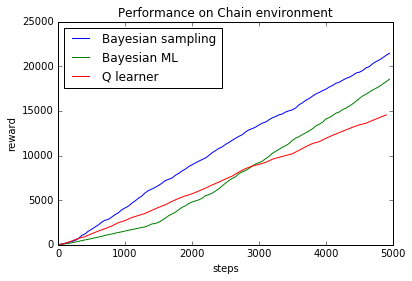
\includegraphics[width=0.48\textwidth]{chainPerf.png}
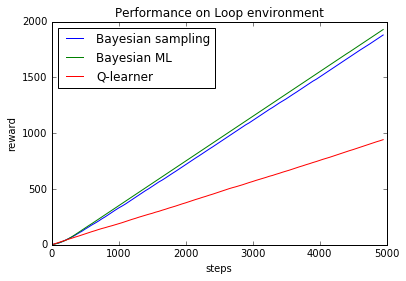
\includegraphics[width=0.48\textwidth]{loopPerf.png}
\caption{\label{fig:chainloopPerf} The performance of three learners in the ``Chain'' and ``Loop''
environments.}
\end{figure}

\begin{figure}[!htb]
\centering
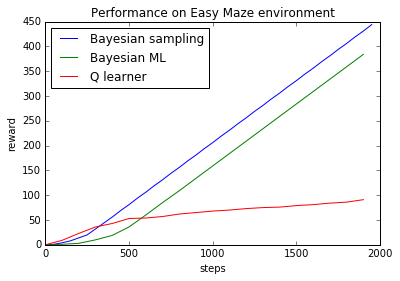
\includegraphics[width=0.48\textwidth]{smallMazePerf.png}
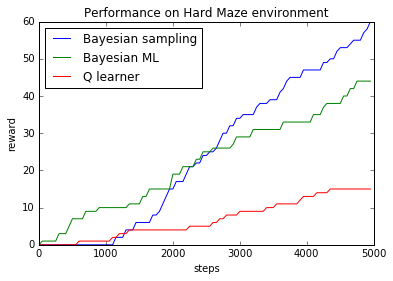
\includegraphics[width=0.48\textwidth]{largeMazePerf.png}
\caption{\label{fig:easyhardPerf} The performance of three learners in the easy and hard ``Maze''
environments. The Bayesian ML and sampling learners clearly outperform the naive $Q$ learner, and
find the optimal policy in the easy maze.}
\end{figure}

In all four environments, the Bayesian ML and sampling learners significantly outperform the naive
$Q$ learner. In the chain environment, the Bayesian sampling learner finds the near-optimal policy and
receives a total reward of 21458, compared with the 18550 from Bayesian ML and the 14548 from $Q$ learning.
The difference between $Q$ and Bayesian models became obvious in the loop problem, in which both Bayesian
sampling and ML achieved optimal performance of staying in the left loop and receiving 2 rewards for every
5 steps, and the $Q$ learner remained in the right loop and received 1 reward for every 5 steps.

In the easy maze problem, the Bayesian sampling learner achieved a near-optimal reward of 456, and both the
Bayesian ML and sampling learners drastically outperform the $Q$ learner. Because our environment provided
so little feedback in the maze, the $Q$ learner was unable to find and exploit the optimal path. The Bayesian
learners were able to deduce the walls without rewards and exploit the optimal path. In the hard maze problem,
all learners struggled, but the Bayesian methods clearly outperform the $Q$ learner. As Figure ~\ref{fig:easyhardPerf}
shows, however, the cumulative reward still sees occasional jumps, indicating it has not converged.

\section{GPSARSA}
In the GPSARSA framework, GPs are used to approximate the quality function $Q$. Similarly to GP regression,
we put a GP prior over $Q \sim \mathcal{N}(0, k(\cdot, \cdot))$, where $\mathbb{E}[Q(x)] = 0$ and
$\mathbb{E}[Q(x)Q(x')] = k(x, x')$, where $x, x' \in \mathcal{X} = S \times A$. The kernel $k(x, x')$
should reflect a similarity notion for the problem at hand.

SARSA refers to the interaction model where $x$ (state-action) is evaluated, a reward is received,
and the new $x'$ is evaluated. We can thus formulate the reward model as
\begin{equation}
R(x^{(t)}, x^{(t+1)}) = Q(x^{(t)}) - \gamma Q(x^{(t+1)}) + N(x^{(t)}, x^{(t+1)})
\label{eq:gpsarsa_R}
\end{equation}
where $N(x, x') = \Delta Q(x) - \gamma \Delta Q(x')$, $\Delta Q \sim \mathcal{N}(0,\Sigma)$,
with $\Sigma(x, x') = \delta(x - x')\sigma^2(x)$. We can define for some time $t$, the random
processes
\begin{align*}
R_t &= (R(x^{(1)},..., R(x^{(t)}))^T \\
Q_t &= (Q(x^{(1)},..., Q(x^{(t)}))^T \\
N_t &= (N(x^{(1)},..., N(x^{(t)}))^T \\
\end{align*}
and the vectors and matrices
\begin{align*}
\mathbf{k_t}(x) &= (k(x^{(1)}, x), ..., k(x^{(t)}, x))^T\\
\mathbf{K_t}(x) &= (\mathbf{k_t}(x^{(1)}), ..., \mathbf{k_t}(x^{(t)}))^T\\
\mathbf{\Sigma_t}(x) &= \textrm{diag}(\sigma_1^2,...,\sigma_t^2)^T.
\end{align*}
$$H^{(t)} =
\begin{bmatrix}
1 & -\gamma & 0 & \ldots & 0 \\
0 & 1 & -\gamma & \ldots & 0 \\
\vdots & \vdots & \ddots & \vdots \\
0 & 0 & \ldots & 1 & -\gamma
\end{bmatrix}$$ and rewrite ~\ref{eq:gpsarsa_R} as

\begin{equation}
R^{(t-1)} = H^{(t)}Q^{(t)} + N^{(t-1)}
\end{equation}

\begin{figure}[!htb]
\centering
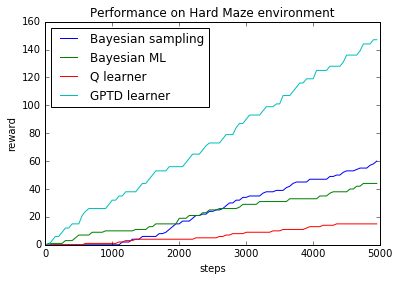
\includegraphics[width=0.48\textwidth]{gptdCompare}
\caption{\label{fig:easyhardPerf} Comparison of GPTD learner against other learners in the hard ``Maze" environment.}
\end{figure}
\begin{figure}[!htb]
\centering
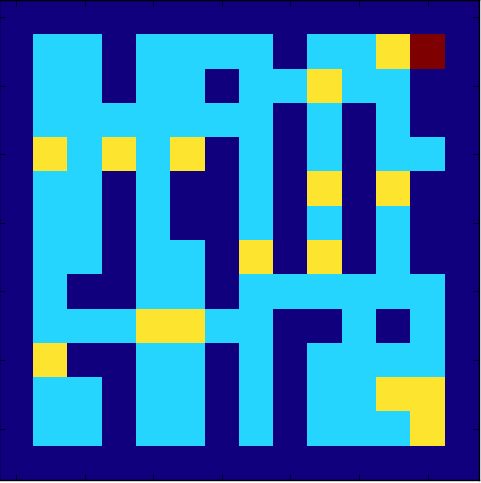
\includegraphics[width=0.30\textwidth]{veryhardmaze}
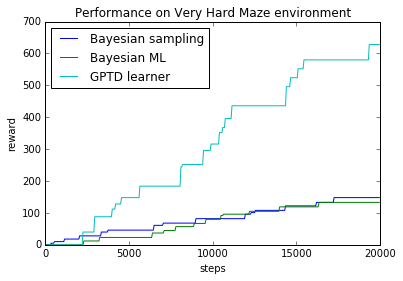
\includegraphics[width=0.48\textwidth]{veryHardMazePerf}
\caption{\label{fig:easyhardPerf} Pictured above is the very hard ``Maze" environment. Pictured below is the performance of GPTD learner against the Bayesian learners on very hard ``Maze" environment.}
\end{figure}

\subsection{Formulation and Experiment}

\section{Source Code}
All of our source code is accessible at \url{https://github.com/alexandrwang/6882project}.

\bibliographystyle{apalike}
\bibliography{writeup}

\end{document}
